%% ==================== document class =========================
\documentclass[11pt]{article}

%% ========================== packages =========================
\usepackage{newpxtext,newpxmath}
\useosf % old-style figures in text, not in math
\linespread{1.05} % Palatino needs a bit more leading than CM
\usepackage[shortlabels]{enumitem}
\usepackage{fancyhdr}
\usepackage{hyperref}
\usepackage{rotating}
\usepackage{setspace}
\usepackage{graphicx}
\usepackage{tabularx}
\usepackage{xcolor}
\usepackage{textcomp}
\usepackage{pgf}
\usepackage[style=numeric,backend=biber]{biblatex}
\addbibresource{bibliography.bib}

%% ========================== document =========================

\begin{document}\thispagestyle{empty}

\pagestyle{fancy}
%... then configure it.
\fancyhead{} % clear all header fields
\fancyhead[RO,LE]{\textbf{SMM638, 2022-23 MTP --- \textcopyright~Simone Santoni}}

\begin{center}
	\textbf{\LARGE SMM638 --- Mid-Term Project}
	
	\vspace{1em}
	
	\textbf{\large Project Package}
	
	\vspace{10em}
	
	\begin{table}[!htbp]
		\begin{small}
			\begin{center}
				\begin{tabular}[c]{|l|l|}
					\hline
					\textbf{Submission deadline} &
					\textcolor{blue}{November 21\textsuperscript{st} at 4:00 PM} \\
					\hline
					\textbf{Template} & Mandatory, available as .docx and .tex format\\
					\hline
					\textbf{Wordl imit} & True, see template documents\\
					\hline
				\end{tabular}
			\end{center}
		\end{small}
	\end{table}

	\vspace{10em}

	\centering

	\textcolor{red}{!! NOT FOR CIRCULATION !!}

	\textcolor{red}{!! DO NOT POST OR SHARE IT!!}

	\vspace{5em}


	\textcopyright~Simone Santoni
\end{center}

\clearpage

\tableofcontents

\clearpage

\section{Project Description}

\subsection{Silico Inc., Company Background}

For this MTP, you will work with real-world data on the R\&D function of a large
company in the industry of semiconductors. Per the non-disclosure-agreement that
is in place, i) I refer to the company with the fictionary name of Silico
Inc., ii) the data do not contain any personal information (e.g., an engineer's
name) and, iii) the distribution of the gender variable  was contaminated by
using synthetic data generation techniques (see Section~\ref{sec:data}).

The R\&D function of Silico Inc. has 19 units --- each of which
is specialized in a field such as microelectromechanical systems, ultra-low-voltage
processors, and rendering --- and includes $1,158$ engineers.  \footnote{All
throughout the various sections of the document, I will use the term engineer
and employee interchangeably.}

The technological innovation process of Silico Inc. is based on 
medium-scale projects whose duration ranges between a few months and one year and a
half. The KPI of a project is the creation of patentable technology. Put
simply, the projects generating a patent are valuable projects for Silico Inc.;
less so, the projects who fail to create a robust and original technology (hence
they do not lead to any patents!).

In terms of organizing, unit heads form small teams of engineers\footnote{The
modal team size is five members. Rarely, teams comprise six or seven members.}
\emph{ad hoc} to work on specific technical issues. At the end of the project,
the teams dissolve and the individual engineers join new projects. 

In terms of process, all Silico Inc. projects follow the same roadmap:

\begin{itemize}
	\item In the first phase, the head of the unit communicates the
	project's technical requirements to the selected group of engineers
	(e.g., reducing  the size of a biosensor\footnote{For basic information
	on biosensors, see~\url{https://en.wikipedia.org/wiki/Biosensor}} 
	currently\footnote{The modal team size is five members. Rarely, teams
	comprise six or seven members.}sold by Silico Inc. of 20\%);
	\item In the second phase, the engineers create a five to ten-page 
	project proposal;
	\item In the third phase, the head of a unit i) evaluates the project 
	proposal against several criteria, ii) provides the team with a
	structured feedback, and iii) decides the project budget;
	\item In the fourth phase, the engineers try to develop a technical
	to the problem identified in the first phase. If the solution
	is robust and original, a patent application is filed for consideration
	by the United States Patent and Trademark Office (USPTO).\footnote{For
	your reference, the USPTO provides an overview of the patenting process
	at~ \url{https://www.uspto.gov/patents/basics/patent-process-overview}.}
\end{itemize}

\subsection{Expectations: Your Role}

Make the following assumptions. First, you are a junior business analyst
working for a global consultancy company. Second, Silico Inc. is your employer's 
client. Third, you are supposed to contribute to
creating a deck to use for a meeting with the client. Specifically,  you are
asked to create a set of network analytic models helping the client to 
improve the performance of the R\&D projects. 

\subsection{Objective}

Your network analytic models should provide actionable insights on how 
to improve the performance of R\&D projects by assembling the right 
team of engineers.
\clearpage

\section{Data}
\label{sec:data}

The client provided you with data on the engineers affiliated with the 19 R\&D
units, the composition and performance of a sample of past projects, and the
network of information exchange between engineers. The data span four files:

\begin{enumerate}[A.]
	\item 
	\texttt{ua.graphml}, reporting the affiliations 
	of employees with the units of the R\&D function of Silico Inc.;
	\item
	\texttt{pa.graphml}, reporting the affiliations 
	of employees with a sample of projects carried out within
	the R\&D function of Silico Inc. recently;
	\item
	\texttt{po.csv}, reporting the performance for a sample of past projects;
	\item
	\texttt{ie.graphml}, reporting the information exchange 
	relationship among the employees of Silico Inc. in the R\&D function
	in the sample.
\end{enumerate}

Table ~\ref{tab:network_data} illustrates the key features of the network data
files mentioned in points A, B, and D. These data are stored in GraphML, a
format based on XML and hence ideally suited as a \textit{``common denominator
for all kinds of services generating, archiving, or processing
graphs.''}\footnote{ See~\url{http://graphml.graphdrawing.org/}} NetworkX has
extensive capabilities to read and write network data in many formats, including
GraphML files. The students are encouraged to refer to the section of NetworkX's
references \texttt{Reading and Writing Graphs > 
GraphML}.\footnote{See~\href{https://networkx.org/documentation/stable/reference/readwrite/graphml.html}
{\texttt{https://networkx.org/.../reference/readwrite/graphml.html}}.}

\begin{sidewaystable}[!hbtp]
	\begin{small}
		\caption{Overview of the Network Data}
		\label{tab:network_data}
		\begin{center}
			\begin{tabular}[c]{l|l|l|c|c}
                        \textbf{Data file} 
			& \textbf{Relationship} 
			& \textbf{Network Form} 
			& \textbf{Node Attributes}
			& \textbf{Edge Attributes}\\
			\hline
			\texttt{ua.graphml}
			& Employee-unit affiliation 
			& Two-mode
			& $\bullet$
			& $\circ$ \\
			\texttt{pa.graphml}
			& Employee-project affiliation
			& Two-mode
			& $\bullet$
			& $\circ$ \\
			\texttt{ie.graphml}
			& Employee-employee information exchange
			& One-mode, undirected
			& $\bullet$
			& $\bullet$ \\
			\hline \\[-1.8ex]
			\multicolumn{5}{l}{\small \textit{Notes.} --- $\bullet$ denotes that the attribute is 
			present in the data file; $\circ$ denotes that the attribute is not
			present in the data file.}
			\end{tabular}
		\end{center}
	\end{small}
\end{sidewaystable}
\clearpage

\subsection{Employee-Unit Affiliation Network}

Per Figure~\ref{fig:ua}, \texttt{ua.graphml} is a two-mode network connecting
1,158 employees to the 19 units in the R\&D function of Silico Inc. Employee
nodes' labels combine the ID of the unit of affiliation and the ID of the
employee (e.g., \texttt{`11-1'}); unit nodes' labels reflect the ID of the units
(e.g., \texttt{`11'}).  The nodes have one attribute, \texttt{bipartite}, 
discriminating between employees (\texttt{bipartite} = $0$), and units 
(\texttt{bipartite} = $1$).

\begin{figure}
	\centering
	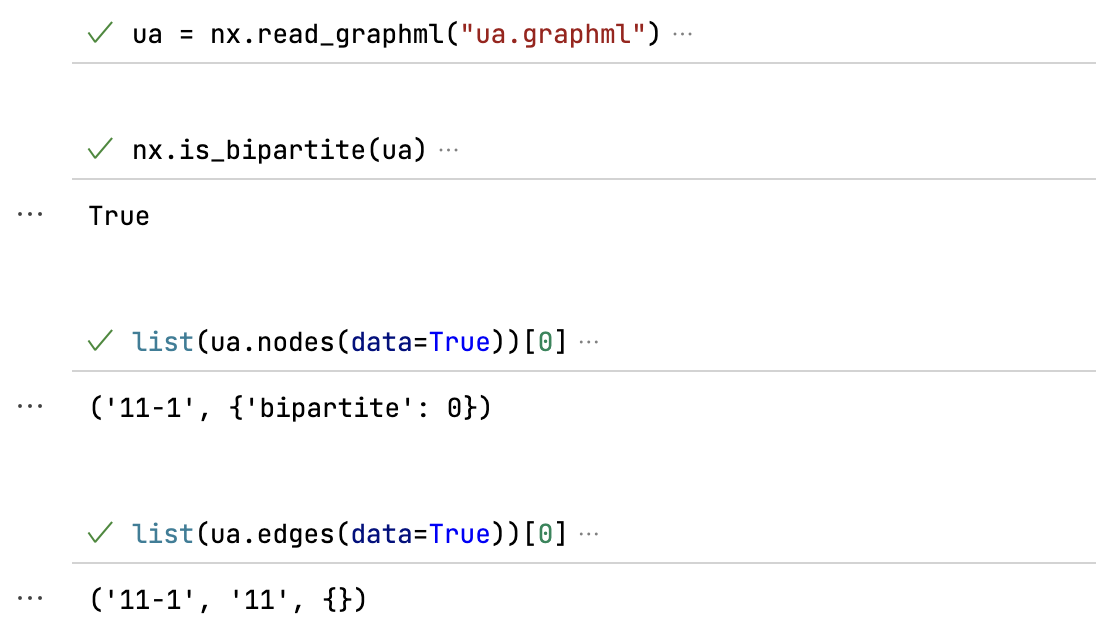
\includegraphics[width=0.95\textwidth]{ua.png}
	\caption{A preview of the attributes of the  
	\texttt{ua.graphml} network dataset}
	\label{fig:ua}
\end{figure}

\subsection{Employee-Project Affiliation Network}

Per Figure~\ref{fig:pa}, \texttt{pa.graphml} is a two-mode network connecting a
665 employees\footnote{It is self-evident from the data that there are 493
employees who are not affiliated with any projects in the sample. The reason is
that, at the time of the data collection, these employees were working on 
ongoing projects for which no outcome was available still.} to the sample of 133
past projects. Project nodes' labels combine the ID of the unit of
affiliation\footnote{In the interest of redundancy, let me stress that the
individual projects are owned by the units of the R\&D function of Silico Inc.}
and the ID of the project (e.g., \texttt{`11-p5'}).  The nodes have one
attribute, \texttt{bipartite}, discriminating between employees (
\texttt{bipartite} = $0$), and projects ( \texttt{bipartite} = $1$).

\begin{figure}
	\centering
	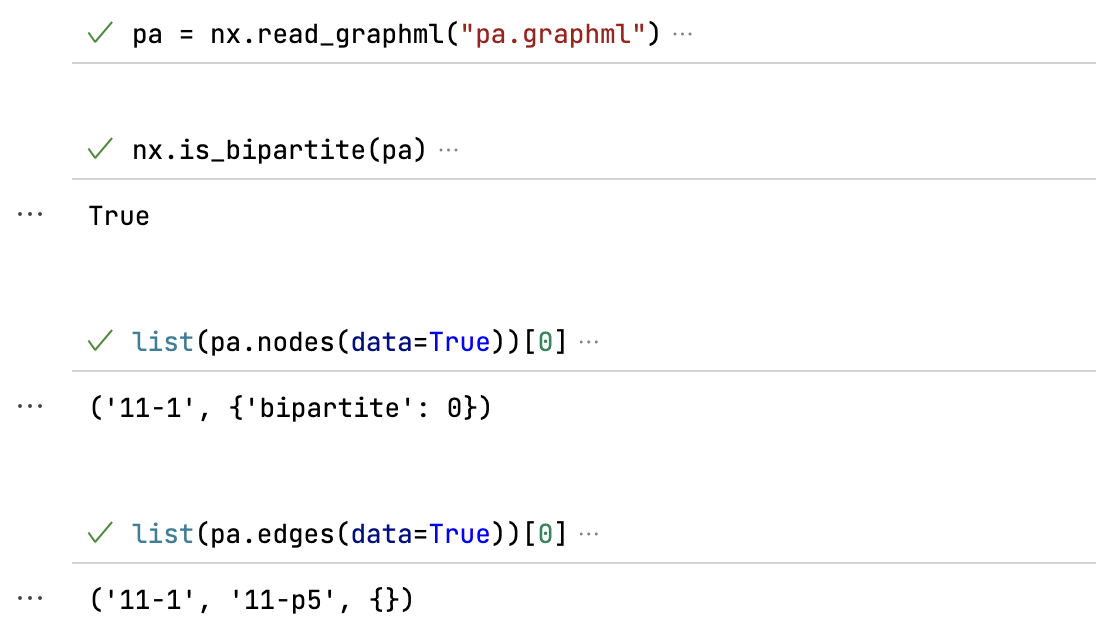
\includegraphics[width=0.95\textwidth]{pa.png}
	\caption{A preview of the 
	 \texttt{pa.graphml} network dataset}
	\label{fig:pa}
\end{figure}

\subsection{Information Exchange Network}

The dataset \texttt{ie.graphml} is a one-mode network connecting 
the 1,158 employees via the information exchange relationship. The data 
come from a survey administered to the population of employees, who were 
asked two things:
\begin{itemize}
	\item To indicate the names of colleagues with whom they shared 
	information on subjects such as technological trends, technical challenges 
	and possible solutions;
	\item To indicate the strength of each tie with the respect to the frequency 
	and intensity of the information exchange.
\end{itemize}

Per Figure~\ref{fig:ie}, each node has three attributes: \texttt{gender} ($0$ = 
female employee; $1$ = male employee), \texttt{ti\_exp}, the technological innovation
experience of employees, measured by the counts of granted patents in which an
engineer `inventor' or `co-inventor', and \texttt{tenure}, the years elapsed since
the employee joined Silico Inc.\footnote{For some employees hired in the 
vicinity of the data collection, \texttt{tenure} is equal to $0$.};  Even the
edges have an attribute in this network: \texttt{strenght} is equal to $0$ for
`weak ties' --- that is, ties with limited frequency and intensity --- and equal
to 1 for `strong ties' --- that is, ties with substantial frequency and
intensity.  Figure~\ref{fig:nviz} illustrates the topology of the
\texttt{ie.graphml} network.

\begin{figure}
	\centering
	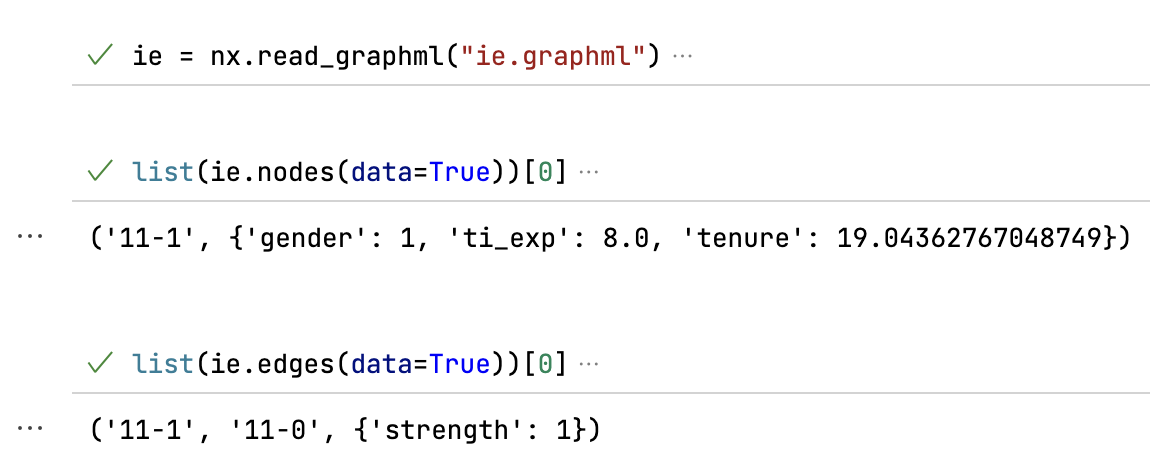
\includegraphics[width=1\textwidth]{ie.png}
	\caption{A preview of the
	 \texttt{ie.graphml} network dataset}
	\label{fig:ie}
\end{figure}

\begin{sidewaysfigure}
	\centering
	\input{graph.pgf}
	\caption{A visualization of the \texttt{ie.graphml} network dataset. 
	\textit{Notes.} --- the color of the nodes reflect the unit 
	of affiliation of the employees; in the interest of simplicity,
	the strength of the ties is not reported in the visualization.}
	\label{fig:nviz}
\end{sidewaysfigure}

\subsection{Project Performance}

Table~\ref{tab:project_performance} indicates the performance measures
for the 133 projects in the sample. The quality of a project proposal 
is assessed by the head of the unit in the third phase of the project's life 
cycle. The patent application is submitted by the unit after the fourth phase 
provided the project generated a robust and novel technological innovation.

\begin{table}[!htbp]
	\begin{small}
		\caption{Project Performance Measures}
		\label{tab:project_performance}
		\begin{center}
			\begin{tabular}[c]{p{5cm}|p{6cm}|p{1cm}}
				\textbf{Measure} 
				& \textbf{Synopsis}
				& \textbf{N}\\
				\hline
				Project proposal quality score\dotfill
				& \quad The score assigned by the head of the unit to the project proposal (out of 100)  
				& 133 \\
				\\[-1.8ex]
				Patent application\dotfill
				& \quad The project generated a patent application 
				($0$ = No, $1$ = Yes)
				& 133 \\ 
				\hline
			\end{tabular}
		\end{center}
	\end{small}
\end{table}


\clearpage

\section{Deliverables}

By November 21\textsuperscript{st}, the students must submit:
\begin{itemize}
	\item  
	An executive summary covering the following aspects
	\begin{itemize}
		\item 
		The main steps of the proposed network analysis;
		\item 
		The justification for each main step;
		\item 
		The main results of the network analysis;
		\item 
		A set of actionable business analytics recommendations 
		grounded in the network analysis results;
	\end{itemize}
	\item
	The Python code necessary to replicate the network analysis
	results reported in the executive summary.
\end{itemize}

The students are required to use the provided template --- available in .docx
and .tex format --- and respect the word limits applying to the various
boxes/sections of the template. The total length of the document is 2,500 words.

\section{References and Contextual Information}

The readings administered  in the third and fourth weeks of the module 
offer a solid knowledge platform to carry out this MTP. 
\textit{Ditto}, the students are welcome to liaise with the module leader about 
further readings and contextual information on the role of networks 
in the management of innovation.

\end{document}